\section{Durchführung}
\label{sec:Durchführung}
Der Versuch besteht aus zwei Teilen, der Synthese und der Analyse der Fuorier-Transformation.
Der Versuchsaufbau zur Synthese besteht aus 4 Geräten. Der Oberwellengenerator erzeugt die Schwingungen, welche zum 
Synthetisieren gebraucht werden. Ein digitales Oszilloskop ist zur Visualsierung der Wellen und späteren Fuorier-Analyse angeschlossen.
Außerdem gibt es einen Scanner, welcher zum Ablesen und Messen der Amplituden genutzt wird, welcher auf einem Funktionen-Erzeuger steht,
mit dem verschieden aussehende Schwingungen erzeugt werden können.
\begin{figure}
    \centering
    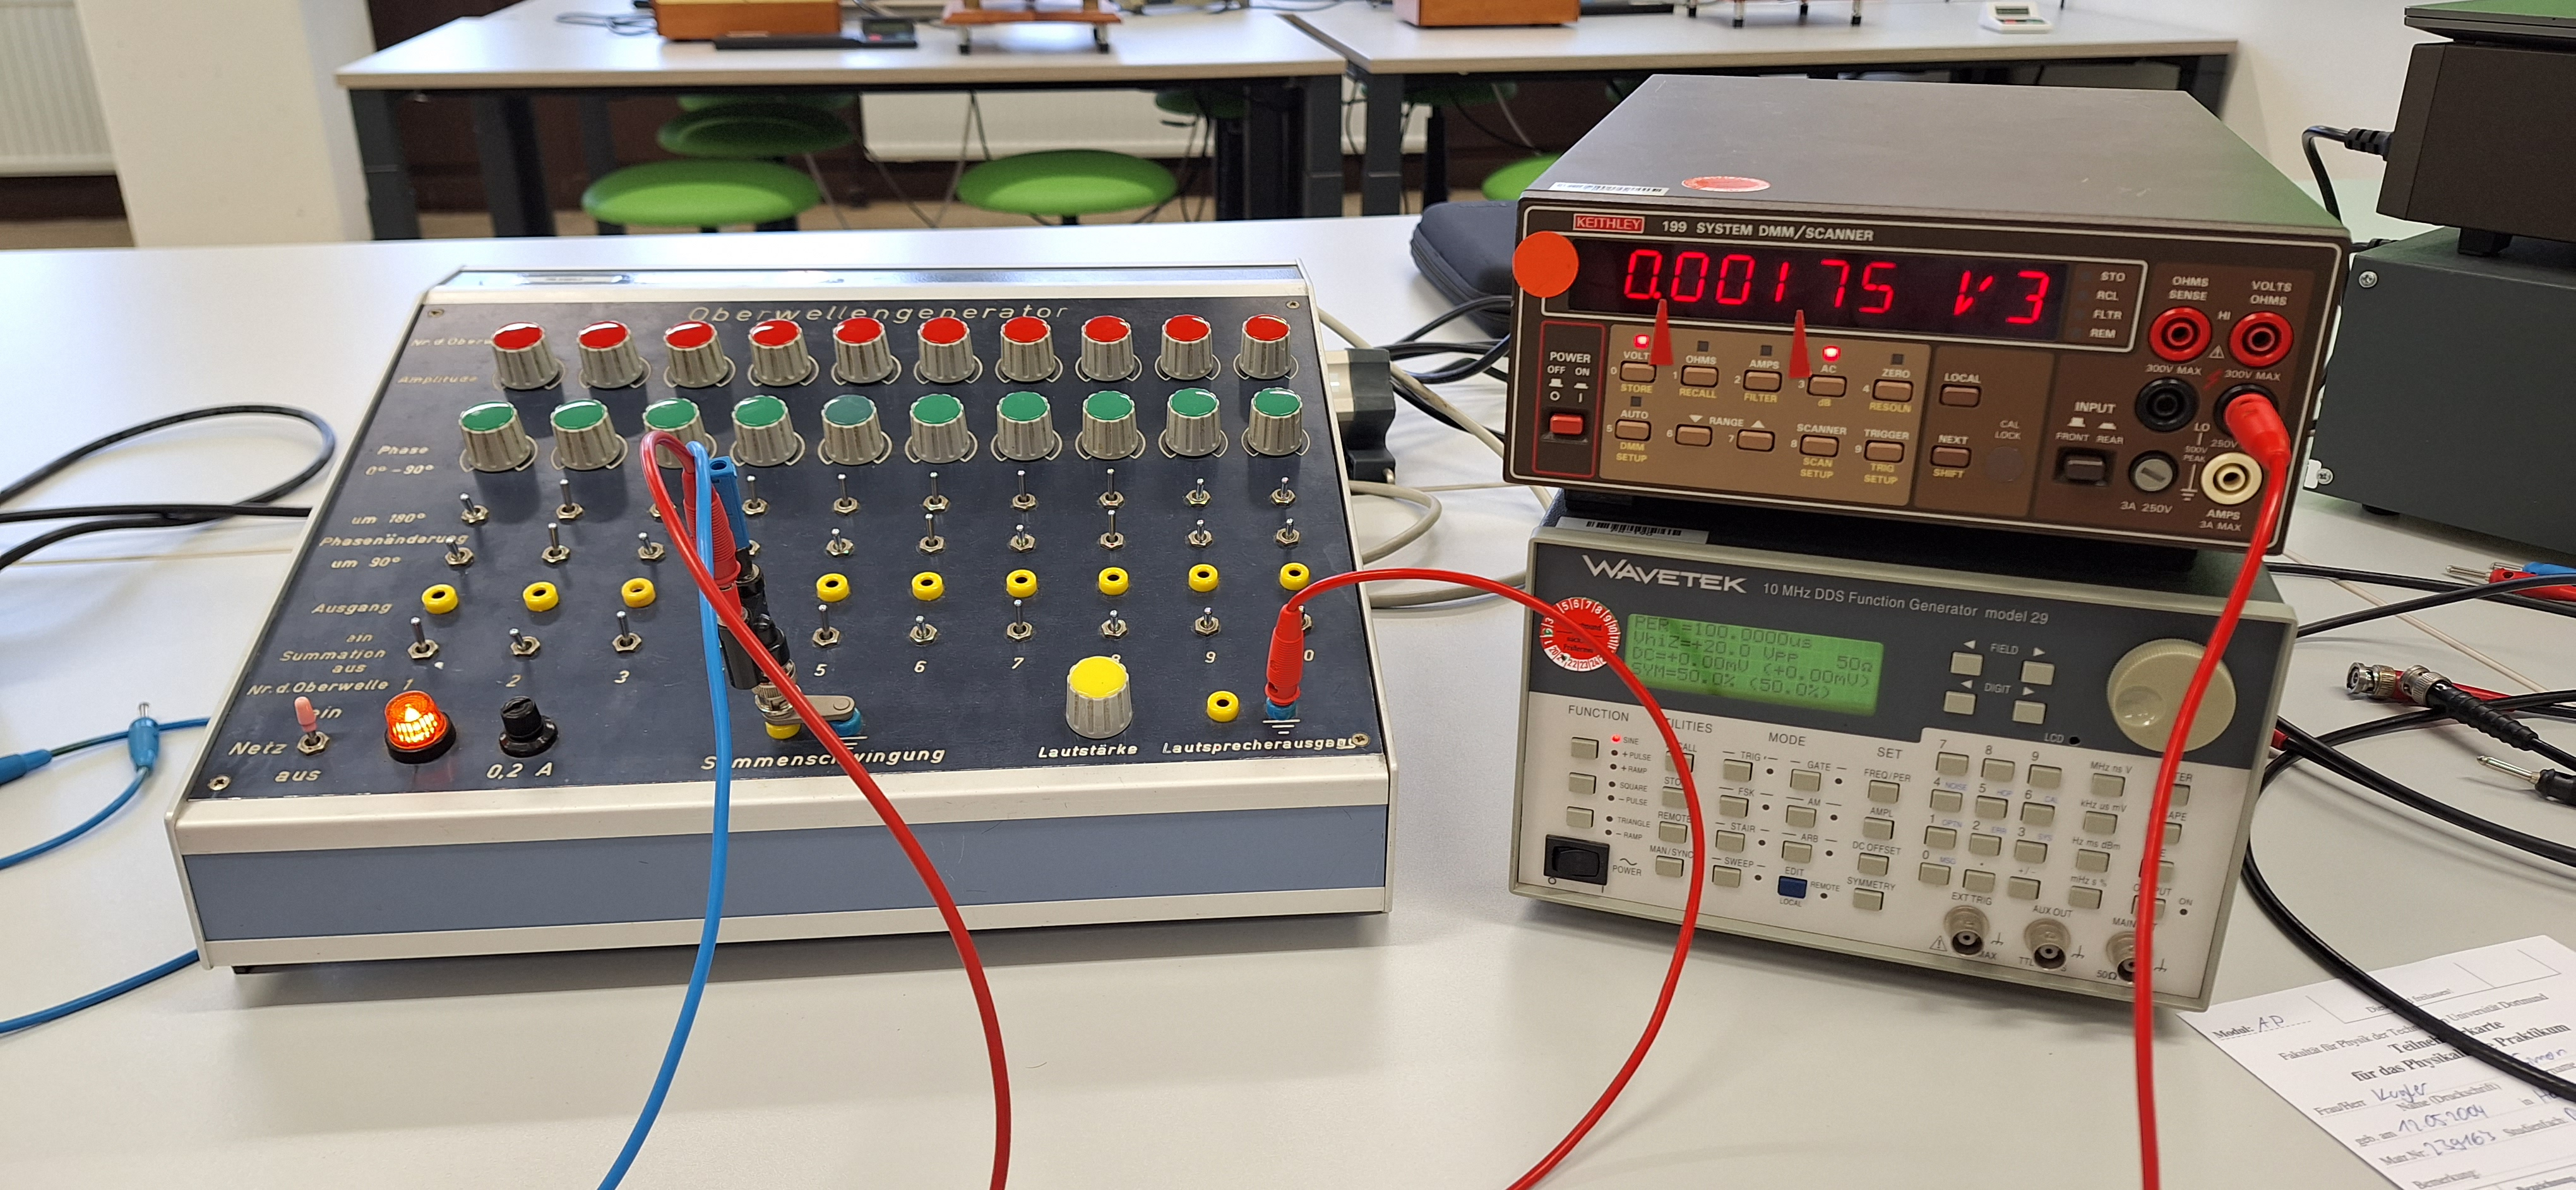
\includegraphics[width=\textwidth]{Messdaten_Bilder/Versuchsaufbau.jpg}
    \caption{Oberwellengenerator, Funktions Erzeuger und Scanner während des Versuchs.}
    \label{fig:Aufbau}
\end{figure}
\subsection{Synthese verschieden aussehender Schwingungen}
Um verschieden aussehende Schwingungen zu synthetisieren, werden mit dem Oberwellengenerator der Oberton sowie verschiedene
Untertöne erzeugt, welche jeweils in verschiedenen Phasen geschaltet eine Dreiecks-, Sägezahn- oder Rechtecksschwingung
ergeben sollen. Um für die Untertöne die richtigen Amplituden zu finden, benötigt man die in der Vorbereitungsaufgabe berechneten 
Koeffizienten. Mit der jeweilig errechneten $\sfrac{1}{n}$-Abhängigkeit wird die Amplitude des Obertons für $n\in\{1,9\}$ durch $n$ dividiert, um 
jeweils die richtige Amplitude für den $n$-ten Unterton einzustellen. Außerdem wird die Phase des Untertons so eingestellt, dass sie mit
dem Oberton übereinstimmt. Dies wird jeweils nur bei den in der Vorbereitungsaufgabe bestimmten $n$-ten 
Untertönen eingestellt, für die die jeweilige Abhängigkeit gilt.
\begin{figure}
    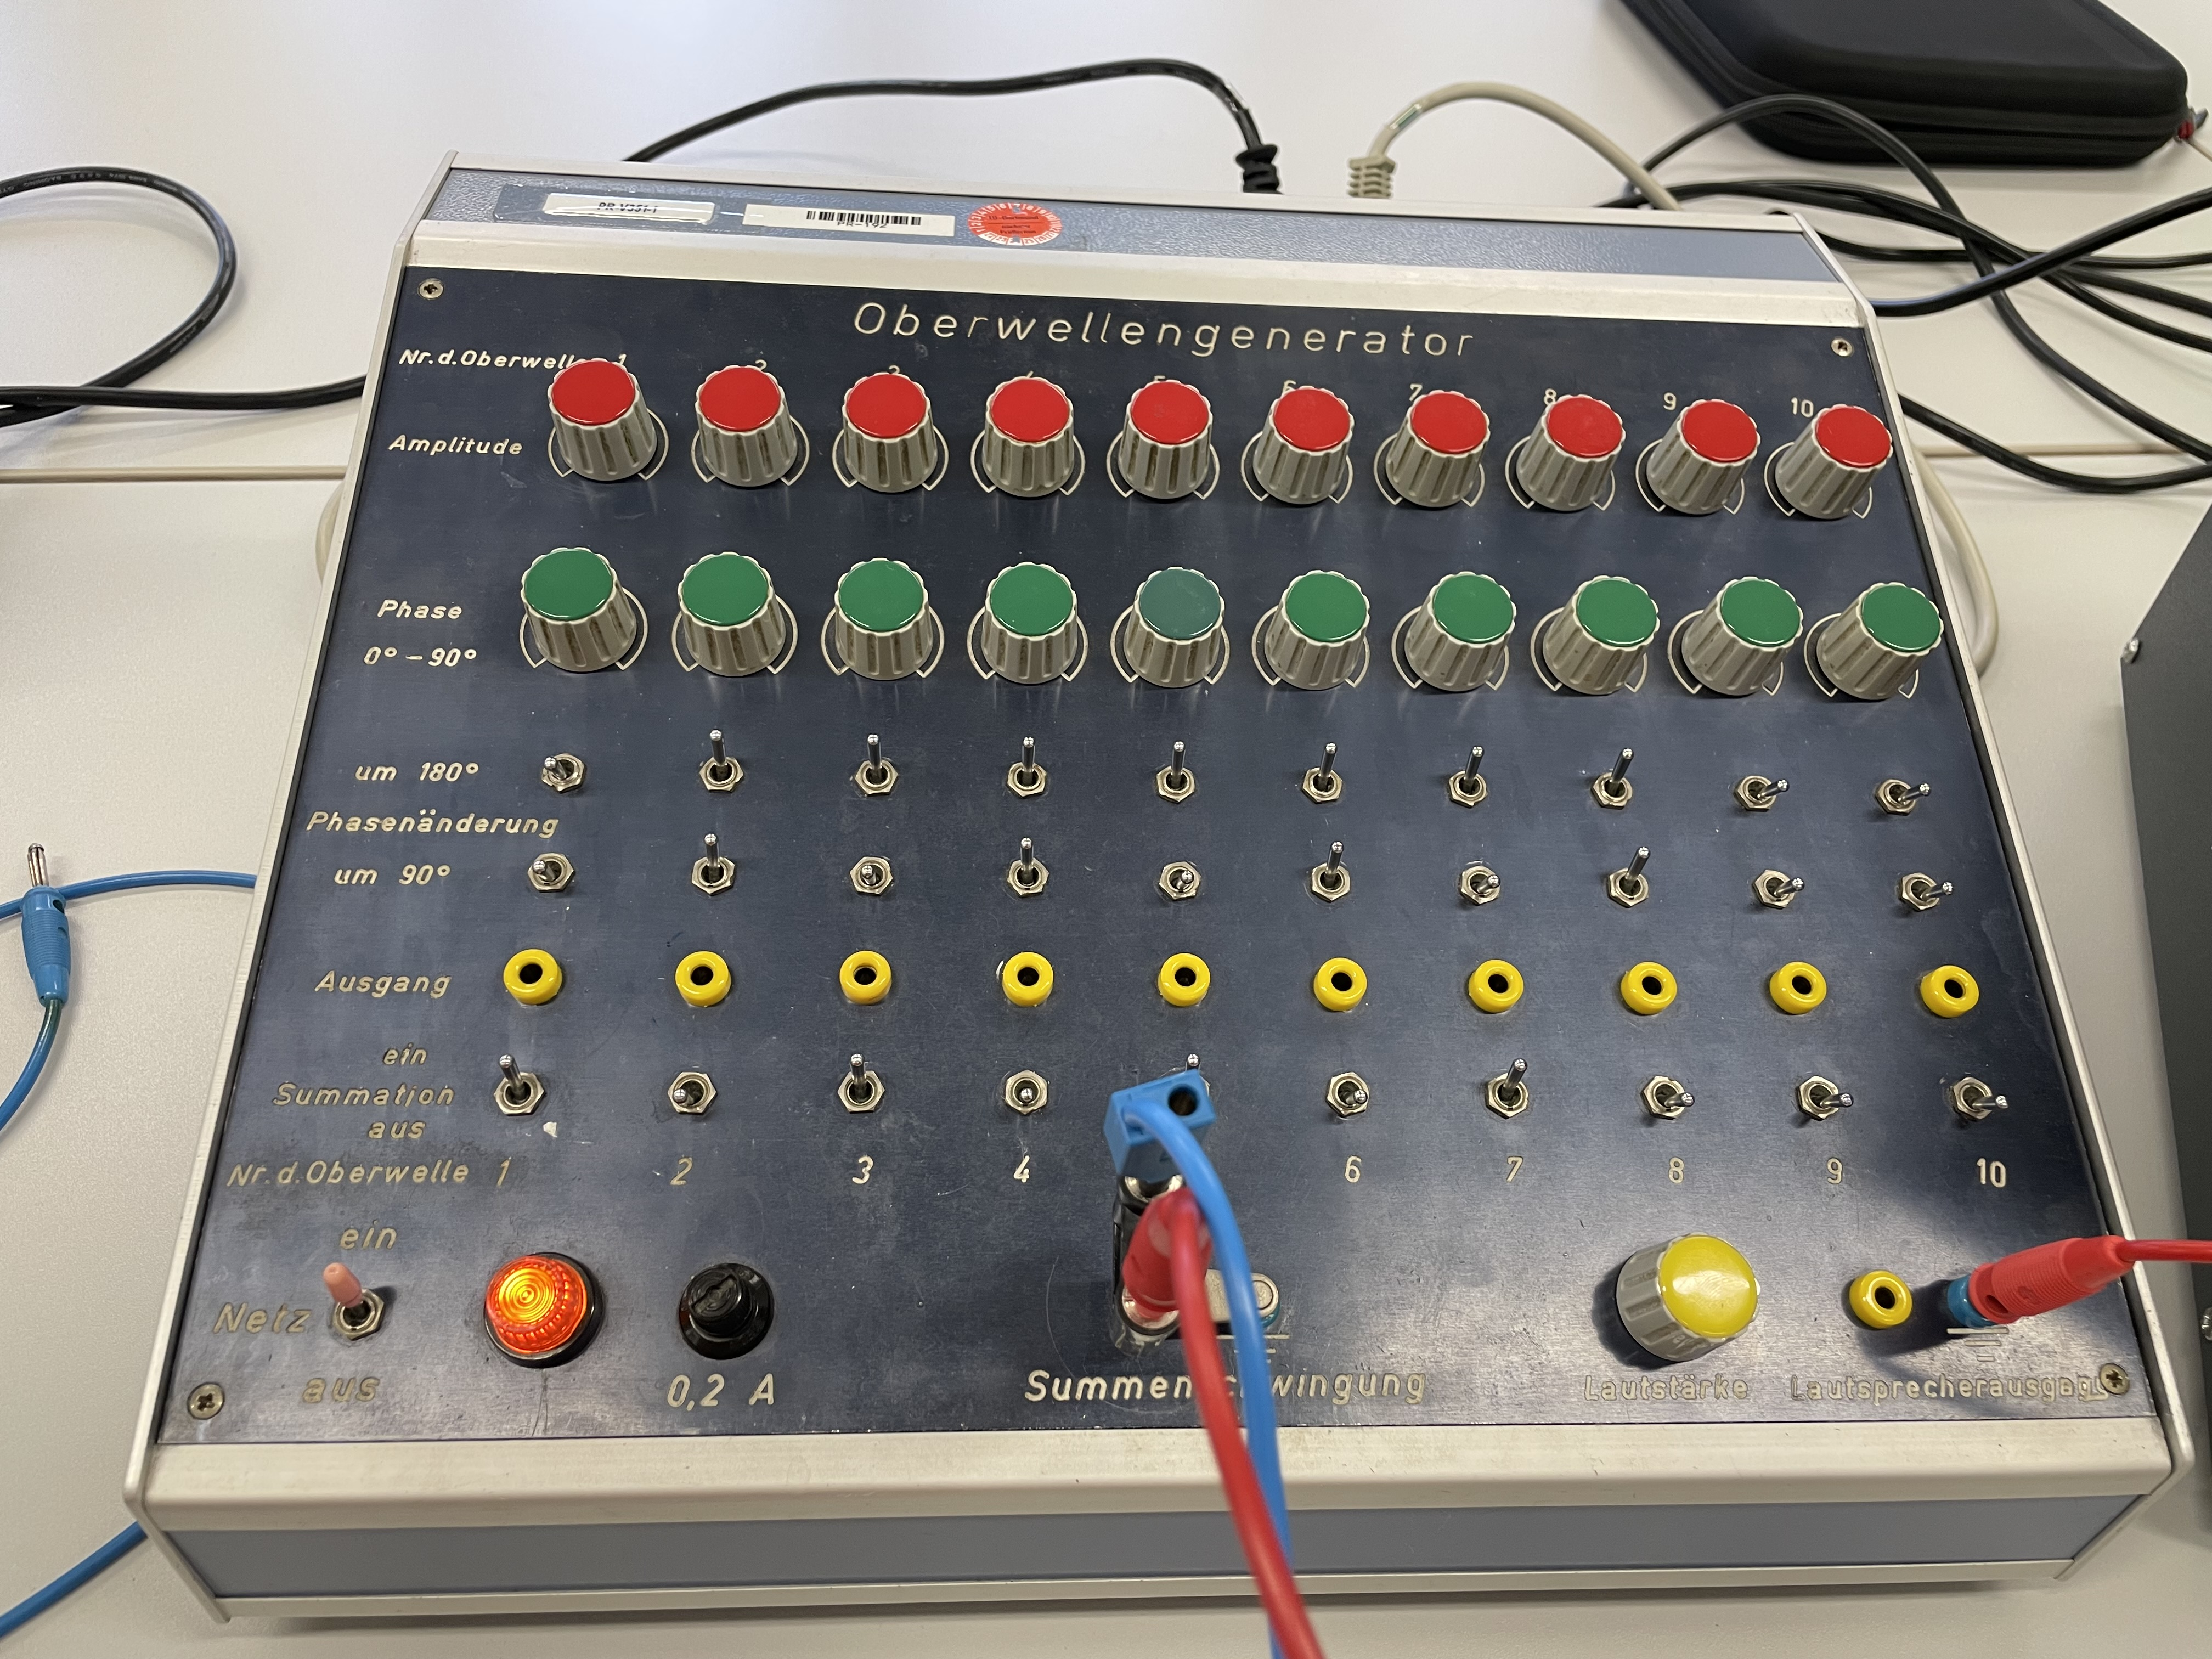
\includegraphics[scale=0.1]{Messdaten_Bilder/Oberwellengenerator.jpeg}
    \caption{Der Oberwellengenerator zum Einstellen der Ober- und Untertöne sowie derer Amplituden und Phasen.}
    \label{fig:Oberwelle}
\end{figure}
\subsection{Fuorier-Analyse}
Es werden am Funktions-Generator verschiedene Schwingungen eingestellt und mit dem Oszilloskop verbunden um sie zu 
visualsieren. Eine Frequenz von 10 000\,kHz wird vorgewählt. Um eine Fuorier-Analyse durchzuführen, muss am Oszilloskop
der Mathe-Modus angewählt und die Einstellung "FFT" für "Fast Fuorier transformation" eingestellt werden. Das Sichtfenster 
und der Frequenz-Teiler werden so eingestellt, dass die Funktion sowie alle Peaks der Zerlegung gut zu erkennen sind um die Messung der Peaks
durchzuführen. Dafür wird ein Courser auf dem Bildschirm eingestellt, mit dessen Hilfe man nach richtigem justieren auf einen Peak
$x$ und $y$ Werte ablesen kann. Der $x$-Wert ist angegeben in kHz, der $y$-Wert in Dezibel. Es werden die Peaks für eine Sägezahn-,
Dreiecks- und Rechtecksschwingung gemessen.
\begin{figure}[H]
    \centering
    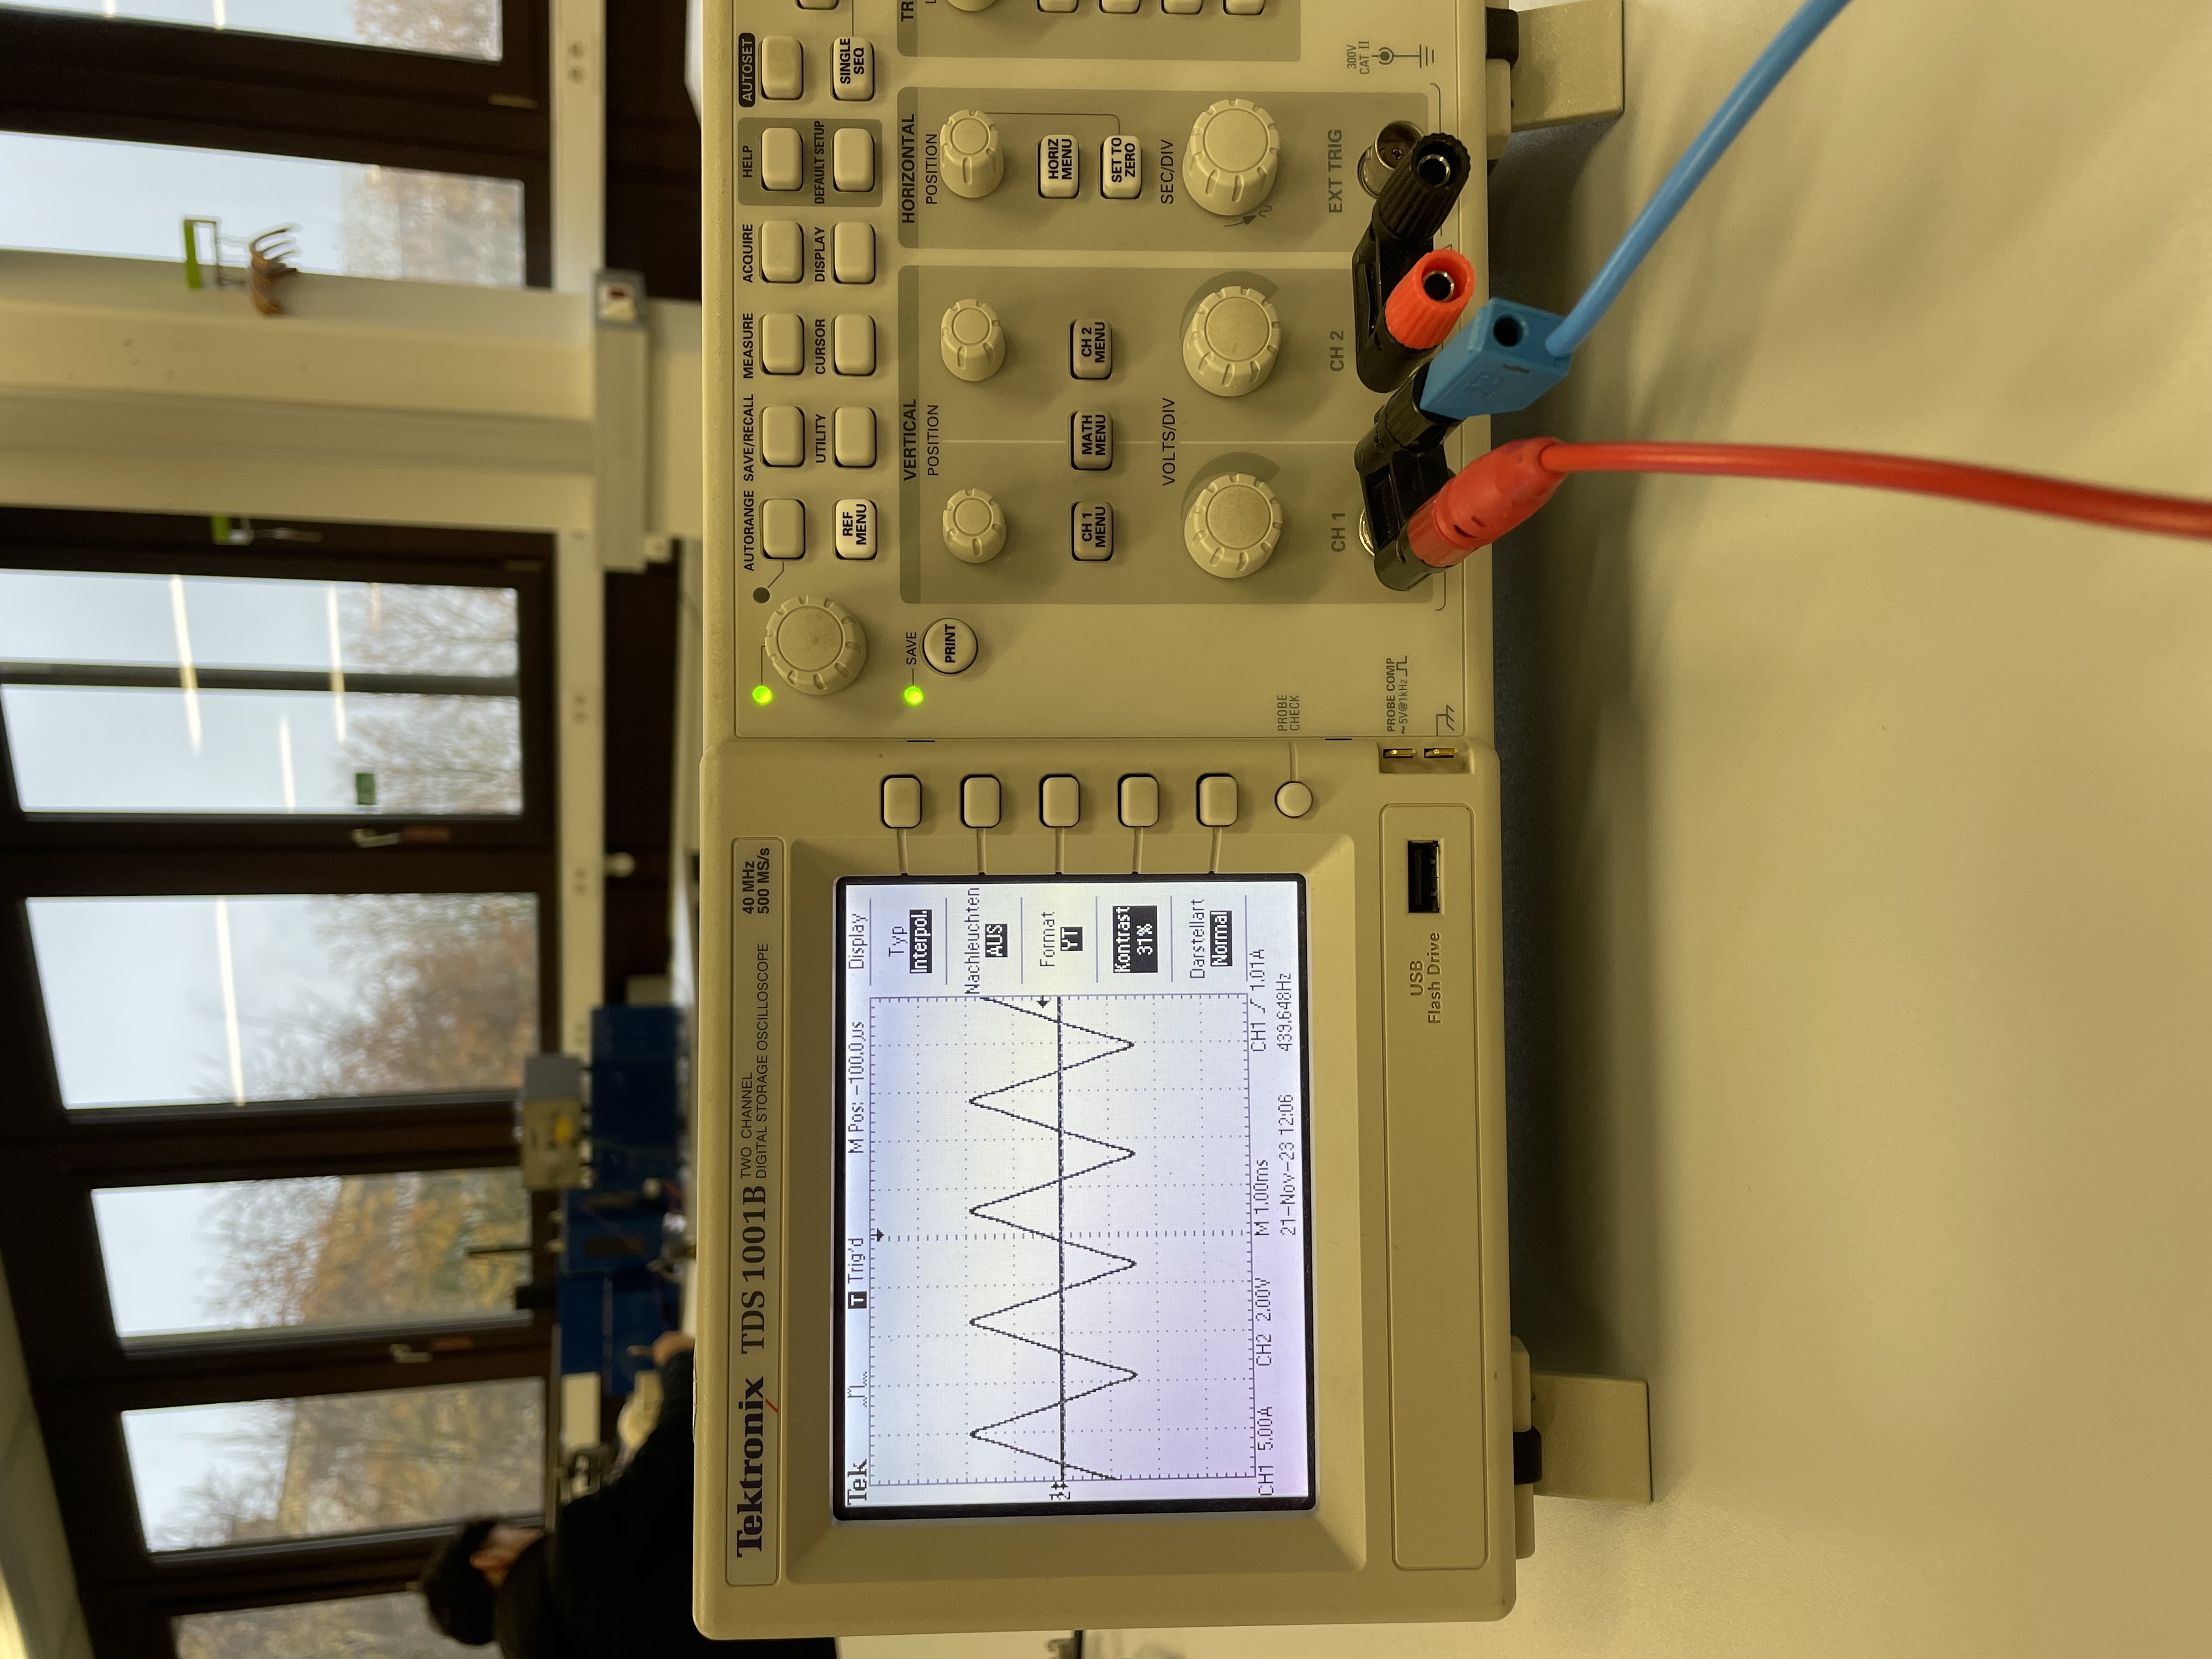
\includegraphics[scale=0.1]{Messdaten_Bilder/Oszilloskop.jpeg}
    \caption{Das zur Fuorier-Analyse verwendete Oszilloskop.}
    \label{fig:Oszilloskop}
\end{figure}